% ****** Start of file apssamp.tex ******
%
%   This file is part of the APS files in the REVTeX 4.1 distribution.
%   Version 4.1r of REVTeX, August 2010
%
%   Copyright (c) 2009, 2010 The American Physical Society.
%
%   See the REVTeX 4 README file for restrictions and more information.
%
% TeX'ing this file requires that you have AMS-LaTeX 2.0 installed
% as well as the rest of the prerequisites for REVTeX 4.1
%
% See the REVTeX 4 README file
% It also requires running BibTeX. The commands are as follows:
%
%  1)  latex apssamp.tex
%  2)  bibtex apssamp
%  3)  latex apssamp.tex
%  4)  latex apssamp.tex
%
\documentclass[%
 reprint,
%superscriptaddress,
%groupedaddress,
%unsortedaddress,
%runinaddress,
%frontmatterverbose, 
%preprint,
%showpacs,preprintnumbers,
%nofootinbib,
%nobibnotes,
%bibnotes,
 amsmath,amssymb,
 aps,
%pra,
%prb,
%rmp,
%prstab,
%prstper,
%floatfix,
]{revtex4-1}

\usepackage{graphicx}% Include figure files
\usepackage{dcolumn}% Align table columns on decimal point
\usepackage{bm}% bold math
%\usepackage{hyperref}% add hypertext capabilities
%\usepackage[mathlines]{lineno}% Enable numbering of text and display math
%\linenumbers\relax % Commence numbering lines
\usepackage{ upgreek }
\documentclass{article}
\usepackage{listings}
%\graphicspath{ {/images} }


\usepackage{amsmath}
%\usepackage[showframe,%Uncomment any one of the following lines to test 
%%scale=0.7, marginratio={1:1, 2:3}, ignoreall,% default settings
%%text={7in,10in},centering,
%%margin=1.5in,
%%total={6.5in,8.75in}, top=1.2in, left=0.9in, includefoot,
%%height=10in,a5paper,hmargin={3cm,0.8in},
%]{geometry}

\begin{document}

%\preprint{APS/123-QED}

\title{Numerical Solutions to the Spherical Harmonic Oscillator Using Eigenvalue Solvers}% Force line breaks with \\

\author{Nicolas Dronchi}
 \altaffiliation[Also at ]{Computational Physics - PHY480}%Lines break automatically or can be forced with \\

\affiliation{%
 Michigan State University\\
 Dronchin@msu.edu \\
 Git Hub link: https://github.com/dronchin/Project2
}%

\date{\today}% It is always \today, today,
             %  but any date may be explicitly specified

\begin{abstract}
Setting up the problem of the three dimensional quantum harmonic oscillator in terms of scaled radial distance variable $\rho$, allows the problem to be solved as a second order differential equation dependent on only one variable. 
The second order finite difference method is used to find the second derivative and the potential of the system is added on to make a tridiagonal Toeplitz matix. Numerical eigenvalues and eigenvectors were found in the non-interacting and interactinge case. The first five eigen values for the non-interacting case were found to be $2.981$, $6.972$, $10.966$, $14.960$, and $18.954$ which is only a \%0.36 error from the expected. For the interacting case, the first five eigenvalues were found to be $4.058$, $7.910$, $11.819$, $15.756$, and $19.708$. The probability for the interacting case matched the predicted pattern of having a large effect at low harmonic oscillator strength. To solve for the eigenvalues both my own Jacobi matrix algorithm was produced as well as the armadillo eig\_sym() function.
\begin{description}
\item[Usage]
Numerical solutions to Schrodinger equation. Jacobi eigenvalue and eigenvector algorithm.

\end{description}
\end{abstract}

\pacs{Valid PACS appear here}% PACS, the Physics and Astronomy
                             % Classification Scheme.
%\keywords{Suggested keywords}%Use showkeys class option if keyword
                              %display desired
\maketitle

%\tableofcontents

\section{\label{sec:level1}Introduction}
\subsection{Buckling Beam}
The starting point of the quantum harmonic oscillator is in the problem of the buckling beam. The similarity is in the initial set up of the differential equation. For the buckling beam the rigidity R and the second derivative of the displacement is related to the force,F, and the displacement,
\[ R \frac{d^2 u(x)}{dx^2} = -F u(x). \]
With the beam being of length L, the problem is a two boundary problem with $u(0) = u(L) = 0$. This problem can be scaled to be proportional to the total length of the beam where $ \rho = x/L $ and $ \rho \in [0,1]$. We get the new equation for the buckling beam:
\[ \frac{d^2 u(\rho)}{d\rho^2} = -\frac{FL^2}{R}u(\rho) = -\lambda u(\rho). \]
This is now an eigenvalue problem where the value of the rigidity can be determined based off of the rigidity. \\
\subsection{Harmonic Oscillator}
The buckling beam is useful because it gives a solvable from for what we want the Schrodinger equation to take. We start with the radial form of the Schordinger equation:
\[ -\frac{\hbar^2}{2 m} \left ( \frac{1}{r^2} \frac{d}{dr} r^2
  \frac{d}{dr} - \frac{l (l + 1)}{r^2} \right )R(r) 
     + V(r) R(r) = E R(r). \]
For the harmonic oscillator we use the potential
\[ V(r) = \frac{1}{2}kr^2 \text{ where } k = m \omega^2\]
because r is defined as the radius from the center we have $r \in [0,\inf)$. We then use the following, 
\[ R(r) = \frac{u(r)}{r} \text{ and assume } l = 0 \]
so that we can substitue and make simplifications to get the radial Schrodinger equation simplified. We get the following after the substitution:
\[ -\frac{\hbar^2}{2 m} \frac{d^2}{dr^2} u(r) + V(r) u(r) = E u(r). \]
In the next step, we introduce a new unitless variable $\rho = r/ \alpha$ where $\alpha$ is a chosen constant with the dimension of length. We also substitute the potential in at this time and simplify the differential equation.
\[ -\frac{\hbar^2}{2 m \alpha} \frac{d^2}{d\rho^2} u(\rho) + \frac{k}{2}\alpha^2 \rho^2  u(\rho) = E u(\rho) 
\]
\[-\frac{d^2}{d\rho^2} u(\rho) + \frac{mk}{\hbar^2}\alpha^4 \rho^2 u(\rho) = \frac{2m\alpha^2}{\hbar^2} E u(\rho) = \lambda u(\rho)\]

We choose \[\alpha = \left \{\frac{\hbar^2}{mk}\right \}^4 \]
So that we are left with a differential equation with a slight variation on the form of the buckling beam that we started with in the beginning.
\[ -\frac{d^2}{d\rho^2} u(\rho) + \rho^2 u(\rho) = \lam u(\rho)
\]
\\

The harmonic oscillator has an analytically solution for the eigenvalues and therefore the energy of the system. The energy of the system depends on an integer n and will follow:
\[ E_n = \hbar \omega (2n + l + 3/2) \]
\\

This is the case of when we have our particles lack interaction and stuck in a harmonic oscillator well. But the question that arrieses next is "what about when the particles are interacting?" \\

\subsection{Interacting Particles}
To Handel the interacting case, we start back at the Schrodinger equation. $r_1$ and $r_2$ are defined, giving the radius between the electron and the center of the system. The Schrodinger equation starting with non-interaction is:
\begin{align*}
\left( -\frac{\hbar^2}{2 m} \frac{d^2}{dr_1^2} -\frac{\hbar^2}{2 m} \frac{d^2}{dr_2^2}+ \frac{1}{2}k r_1^2+ \frac{1}{2}k r_2^2\right)u(r_1,r_2) \\
= E^{(2)} u(r_1,r_2) .
\end{align*}


Then we define $r = r_1 - r_2$ and $R = 1/2*(r_1 + r_2)$ which will allow us to define Schordinger's equation in terms of center of mass coordinates. We get the following equation,
\begin{align*}
\left( -\frac{\hbar^2}{m} \frac{d^2}{dr^2} -\frac{\hbar^2}{4 m} \frac{d^2}{dR^2}+ \frac{1}{4} k r^2+ kR^2\right)u(r,R)\\
= E^{(2)} u(r,R).
\end{align*}

We split the energy that we're looking at and therefore the equation into two parts by using the relation that $u(r,R) = \psi(r) \phi (R)$. This splits the energy into $E = E_r + E_R$. Because we are only interested in the potential for systems with $l=0$, we can ignore the center of mass energy. We also add on a part of the coulomb interaction potential. We add on the potential,
\[ V(r_1,r_2) = \frac{\beta e^2}{|\mathbf{r}_1-\mathbf{r}_2|}=\frac{\beta e^2}{r},
\]
with $\beta e^2=1.44$ eVnm. \\

With the new potential and seperation of energies, we obtain the following equation:
\[ \left( -\frac{\hbar^2}{m} \frac{d^2}{dr^2}+ \frac{1}{4}k r^2+\frac{\beta e^2}{r}\right)\psi(r) = E_r \psi(r). \]
With this we do the same unitless variable transformation done in the harmonic oscillator case for $\rho = r/\alpha$ and we combine a few other variables to clean up the expression. We define the following:
\begin{align*}
\omega_r^2=\frac{1}{4}\frac{mk}{\hbar^2} \alpha^4 \ \ \ \lambda = \frac{m\alpha^2}{\hbar^2}E\\
\alpha = \frac{\hbar^2}{m\beta e^2} \ \ or \ \ \frac{m\alpha \beta e^2}{\hbar^2}=1.
\end{align*}
Using these new definitions we can finally write the Schrodiner equation in a form that is familiar and consistent with the one observed in the harmonic oscillator.
\begin{align*}
 -\frac{d^2}{d\rho^2} \psi(\rho) + \omega_r^2\rho^2\psi(\rho) +\frac{1}{\rho} = \lambda \psi(\rho).
\end{align*}
\\

The large difference comes with the new $1/\rho$ term that is added to the potential while the $\omega_r$ reflects the strength of the harmonic potential that the particle interacts in. In strong harmonic potentials, the $1/\rho$ term will be small in comparison not make a significant difference. In the presence of a weak harmonic oscillator potential, the $1/\rho$ term will dominate and produce a significant difference from the non-interacting case. \\

%Maybe add an intro to what I solved for?

\section{\label{sec:level1}Methods and Implementation}
\subsection{Tridiagonal Toeplitz Setup}
The first order finite difference method is defined as 
$$ u'(x) = \frac{u(x+h) - u(x)}{h} + O(h)$$
where the error $O(h)$ is scaled with the size of the step size h. [2,3]\\

Here we use the second order finite difference method, which is defined as
$$ u''(x) = \frac{u(x+h) + u(x-h) - 2u(x)}{h^2} + O(h^2)$$
where the error $O(h^2)$ is scaled with the square of the step size h.\\

The solution of this problem begins with a change of variables to $\rho$ so that the function is discretized at specific points. For a set number of points N, $\rho_{min}$, and $\rho_{max}$ we calclate the step interval $h$,
\[ \frac{\rho_{max} - \rho_{min}}{N} = h.  \]
The discretized values of $\rho$ are then defined by $\rho_i = \rho_{min} + h*i$ for $i = 1,2,...,N$. With $\rho$ discretized, you discretize the finite differece method along with it so that you get $$u_i'' = \frac{u_{i+1} + u_{i-1} - 2u_i}{h^2} \hspace{10mm} for \hspace{10mm}  i = 1,2,..., N$$
Because of how the boundary conditions were defined, we have to pick a max $\rho$ value to solve up to so that $u(0) = 0$ and $u(\rho_{max}) \approx 0$, and we set up $A$, an $nxn$ matrix. In the case of the buckling spring problem stated in the intro, the main diagonal elements $d_i = 2$ and the off diagonal elements $e_i = -1/h^2$. This makes the matrix $A$ equal to the following:
$$ A =
\begin{bmatrix}
    2 & -1 & 0 & \dots & \dots & 0 \\
    -1 & 2 & -1 & 0 & \dots  & \dots \\
    0 &-1 & 2 & -1 & 0  & \dots \\
    0 & \dots & \ddots & \ddots & \ddots & 0 \\
    0 & \dots & \dots& -1 & 2 & -1 \\
    0 & \dots & \dots & \dots& -1 & 2
\end{bmatrix} $$
 b is a matrix equal where $b_i = \frac{-FL^2}{R}u_i$ and x is the solutions to the second order derivative to $u_i$ at the discretized values of $x_i$. This system of equations is changed so that the potential is added on for the harmonic oscillator with and without interaction.\\
 
 For the harmonic oscillator potential, when the problem is discretized, we get the same approximation for the second derivative except the potential is added on at discretized values. The discretization of the derivative at different values of $\rho_i$ are formed from the following:
 \[
-\frac{u_{i+1} -2u_i +u_{i-1} }{h^2}+V_iu_i  = \lambda u_i,
\]
\\

This makes the values for the diagonal elements for the tridiagonal Toeplitz matrix,
\[ d_i = 2/h^2 + V_i \ \ \ \  where \ \ V_i = \rho_i^2 \ \ or \ \ V_i = \omega^2\rho_i^2 +1/\rho_i \]
depending on whether or not the particles are interacting. The off diagonal elements stay the same where $e_i = -1/h^2$ making the new matix $A$ used in the eigenvalue solver.

\subsection{Eigenvalue Solver}
In this project two methods of eigenvalue solvers were used. The first being an eigenvalue solver that was self created using the Jacobi method of finding eigenvalues and the other using the armadillo library's eig\_sym function. \\

The eigenvalue solver in armadillo actually just calls the lapack eigenvalue solver. The lapack solver depends on the version you're using but for verson 2, it uses the xSTEDC algorithm. The details on how the algorithm works and other algoritms used by lapack in different versions can be found at the following: http://www.netlib.org/lapack/lug/node70.html \\

For my eigenvalue solver, the Jacobi method was used. The Jacobi method takes in a dense matrix and creates a diagonal matrix with the eigenvalues stored along the diagonal after many loops. The number of loops isn't explicit and depends on the properties of the matrix being examined. For each loop, the largest off diagonal element is located. If that element is larger than some set limit on accuracy, $\epsilon$, then a similarity transformation is applied on that matrix. After some number of similarity transformations are applied, the off diagonal elements get smaller and smaller so that they are as close to zero as possible to compute within a limit of time. The general loop is set up in my code that can be seen bellow. \\

\begin{lstlisting}[language=c++, caption=Jacobi method]
int jacobi(int n, mat &A, mat& v){
  double max;
  double eps = 1e-8;
  double maxiter = (double)(n*n*n);
  int k = 0; int l = 0;

  max = maxoffdiag(A,n,&k,&l);
  int iter = 0;
  while(fabs(max) > eps && 
  (double) iter < maxiter){
    max = maxoffdiag(A,n,&k,&l);
    rotate(A,v,n,k,l);
    iter++;
  }
  return 0;
}
\end{lstlisting}

In listing 1, the rotate() function takes in the location of the largest max diagonal element and preforms a similarity transformation of a rotation matrix.  For the similarity transformation, a $nxn$ matrix S is created is similar to the identity matrix except that the values at
\[ s_{kk} = s_{ll} = \cos{\theta}, s_{kl} = -s_{lk} = -\sin{\theta} \]
Take an example where the max off diagonal element is found at $(3,5)$ in a $6x6$ matrix. This results in creation of a matrix that look like the following:
\[ A =
\begin{bmatrix}
    1 & 0 & 0 & 0 & 0 & 0 \\
    0 & 1 & 0 & 0 & 0  & 0 \\
    0 & 0 & \cos{\theta} & 0 & \sin{\theta}  & 0 \\
    0 & 0 & 0 & 1 & 0 & 0 \\
    0 & 0 & -\sin{\theta} & 0 & \cos{\theta} & 0 \\
    0 & 0 & 0 & 0 & 0 & 1
\end{bmatrix} \]
To calculate the next matrix in the loop $B$, you apply the similarity transformation as
\[ B = S^T A S \]. \\

The trick is finding out which angle to rotate the matrix at and then applying the rotation based off of the calculated $\sin{\theta} = s$ and $\cos{\theta} = c$. To do this we follow this general path: 
\begin{enumerate}
  \item Calculate $\tau$, where $\tau = (a_{kk}- a_{ll})/(2*a_{kl})$ 
  \item Calculate $\tan{\theta} = t$ using the fact that $t^2 +2\tau t - 1 = 0$
  \item Calculate $sin$ and $cos$ using $c = 1/\sqrt{1+t^2}$ and $s = t*c$
  \item Replace new values of $a_{kk}=a$ and $a_{ll}$: $a_{kk} = a_{kk}c^2 + a_{ll}s^2 - 2 c s a_{kl}$ and $a_{ll} = a_{kk}s^2 + a_{ll}c^2 + 2 c s a_{kl}$
  \item Set $a_{lk} = a_{kl} = 0$
  \item Loop through and preform rest of matrix multiplication on every element that isn't $a_{lk}, a_{kl}, a_{kk}, or a_{ll}$
\end{enumerate}

To find the eigenvectors along side, you preform the same similarity transformations on an initial identity matrix. This gives normalized eigenvectors in which the columns correspond to the eigenvalue in the order of the diagonal. 

\subsection{Unit Tests}
As part of the calculations, unit tests were created along side my functions to test their results. The unit tests I chose to include are: "Testing maxoffdiag of A(i,j)", "Testing eigenvalues from jacobi", "Rotate preserves frobenius norm", and "Eignvector orthoganality". Each test was preformed using Catch, an open source C++ project that can be found at https://github.com/catchorg/Catch2. \\

For the maxoffdiag, the tridiagonal Toeplitz matrix is created of size 5x5. A random location not on the diagonal is chosen and a very large value is put in that location. The maxoffdiag is then run on the matix and the location it returns is compared to the location the value was put on. \\

For the testing eigenvalues unit test, the tridiagonal Toeplitz matrix creates 2 inital matricies and my jacobi eigenvalue solver is ran as well as the armadillo eig\_sym function is run. The eigen values from both of these methods are then compared to be within a given accuracy.\\

For the Rotation preserving the Frobenius norm, The Frobenius norm was calculated before a rotation was created on the tridiagonal Toeplitz and after the rotation function was used on it. The Frobenius norm is calculated as $||A|| = \sqrt{\sum_i^N\sum_j^N |a_{ij}|^2}$ and is conserved through all similatrity transformations. \\

Finally, for the vector orthoganality, I created a 4x4 matrix and solved for it's eigenvalues and eigenvectors using eig\_sim(). The dot product of the columns were then taken and shown to equal zero. 


\section{\label{sec:level1}Results and Analysis}


The eigenvalues obtained from the non-interacting harmonic oscillator were $2.98198$, $6.97287$, $10.966$, $14.9601$, $18.9549$. These were obtained from using $N=1000$, $\omega = 1$, and $\rho_{max} = 6$. This is compared to the analytical eigenvalues of $\lambda = 3,7,11,15,19$. The eigenvectors from the first three energies are plotted bellow in firure \ref{fig:wavefunctions} as the radial wavefunctions and then in figure \ref{fig:probabilites} the probabilities.\\

\begin{figure}[h]
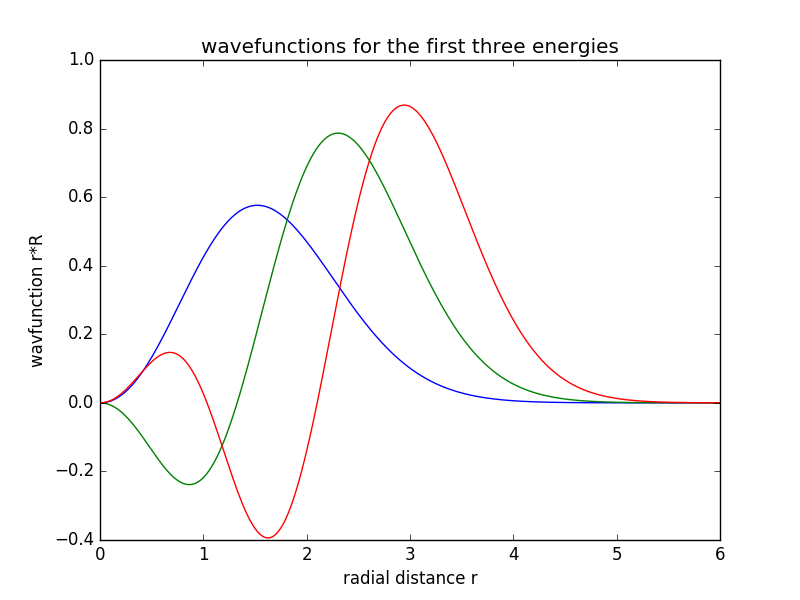
\includegraphics[width=\linewidth]{3wavefunctions.png}
\caption{normalized wavefunctions for the first 3 energies of the non-interacting case. The eigenvectors were muliplied by the r values and then plotted against the r values.}
\label{fig:wavefunctions}
\end{figure}
\begin{figure}[h]
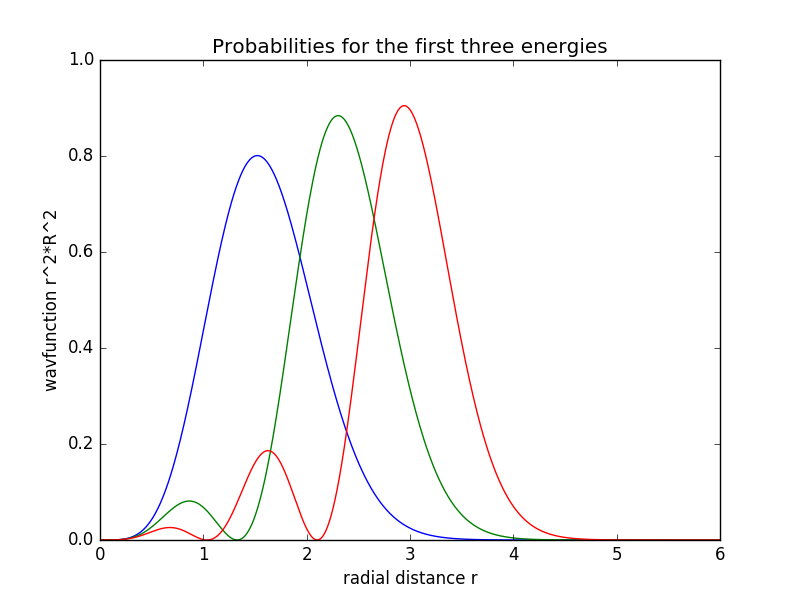
\includegraphics[width=\linewidth]{3probabilities.png}
\caption{Normalized probabilites for the first 3 energies of the non-interacting case}
\label{fig:probabilites}
\end{figure}

The conversion of these eigenvalues back to real values comes with the relation back to energy. Back in the intro section, a substitution to $\lambda$ was made. We have the relationship
\[ \frac{2m\alpha^2}{\hbar^2} E = \lambda \]
we also know that 
\[\alpha = \left \{\frac{\hbar^2}{mk}\right \}^4 \]
Therefore through simplficaiton we find how to bring our numerical answer back to numbers that will match experimental values. 
\[ E = \frac{\hbar}{2}\omega \lambda\] \\

The next case to look at is the interacting case. With the same conditions as the non-interacting case were $N=1000$, $\omega = 1$, and $\rho_{max} = 6$, we get that the eigenvalues are $4.05785$, $7.90959$, $11.819$, $15.7557$, and $19.7079$. With high values of $\omega$, we expect that the interacting and non-interacting case are consistent with each other. It's only at low values of $\omega$ that we see the $1/\rho$ term start dominating. \\

For different values of $\omega$ balancing the starting variables of $N$ and $\rho_{max}$ become important. If $N$ is too small, you start to lose numerical precision in your answer. If $N$ gets to big, you quickly approach program run times that become unreachable. I found the right ballance between precision and runtime to be about $N = 1000$ for my setup. For $\rho_{max}$, it depends on the $\omega$. For low values of $\omega$, you need a higher $\rho_{max}$. For the case of $\omega = 5$, $1$, and $0.5$, a $\rho_{max} = 6$ is sufficient. For the case of $\omega = 0.01$ a $\rho_{max} = 40$ was needed.\\

The interacting vs non-interacting case can be seen summarized in the following figures 3-7.
\begin{figure}[h]
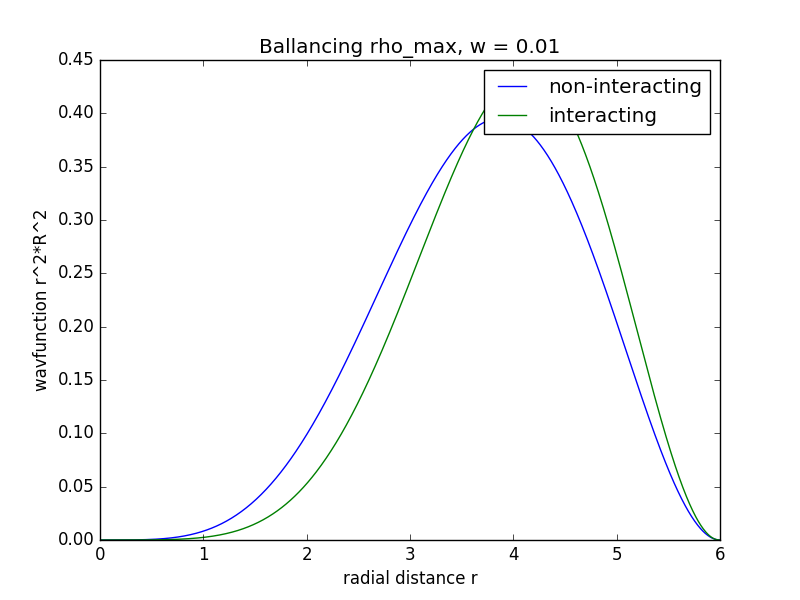
\includegraphics[width=\linewidth,height=130pt]{ballancingrho_max_final.png}
\caption{Effect of low $\rho_{max}$}
\label{fig:bad}
\end{figure}


\begin{figure}[p]
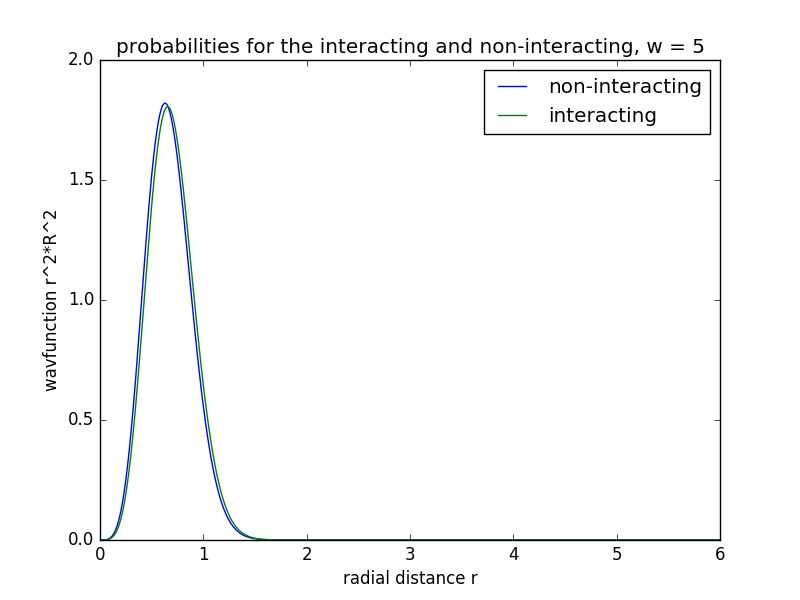
\includegraphics[width=\linewidth,height=130pt]{intervsnon_w5_final.png}
\caption{Probabilities for interacting vs non-interacting, w=5}
\label{fig:w5}
\end{figure}

\begin{figure}[p]
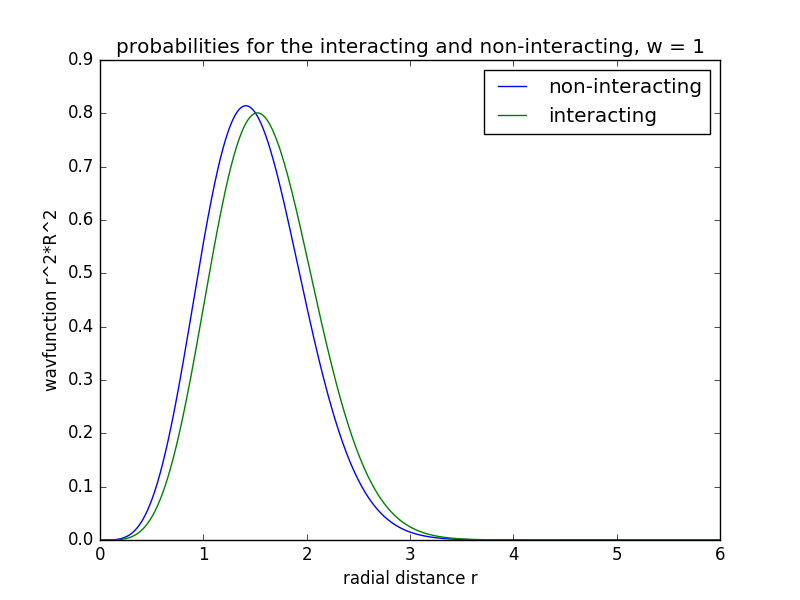
\includegraphics[width=\linewidth,height=130pt]{intervsnon_w1_final.png}
\caption{Probabilities for interacting vs non-interacting, w=1}
\label{fig:w1}
\end{figure}

\begin{figure}[p]
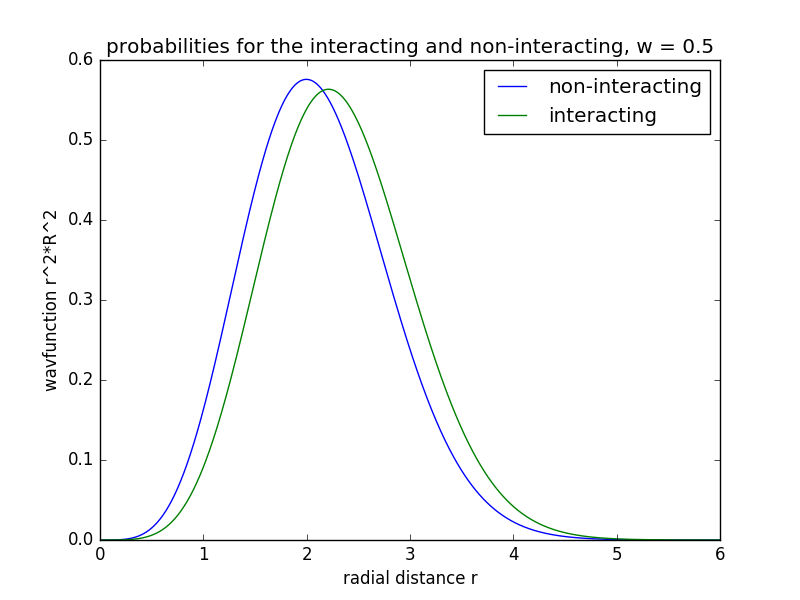
\includegraphics[width=\linewidth,height=130pt]{intervsnon_w05_final.png}
\caption{Probabilities for interacting vs non-interacting, w=0.5}
\label{fig:w05}
\end{figure}

\begin{figure}[p]
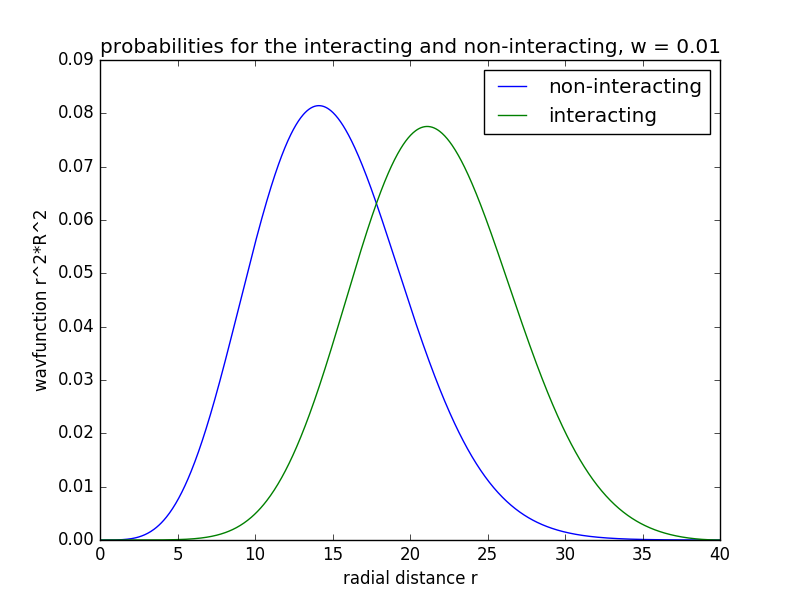
\includegraphics[width=\linewidth,height=130pt]{intervsnon_w001_final.png}
\caption{Probabilities for interacting vs non-interacting, w=0.01}
\label{fig:w001}
\end{figure}


For figures \ref{fig:w5}, \ref{fig:w1}, \ref{fig:w05}, and \ref{fig:w001}, we see the predicted effect that as $\omega$ increases, the more the $1/\rho$ factor comes in to play. For \ref{fig:w5}, the two lines are practically overlapping and it is hard to see the difference between them. for \ref{fig:w001} there are very distinct lines with the interacting case having it's probability farther out from the center. \\

Finally, it is important to talk about the eigenvalue solver efficiency. My jacobi matrix solver would not solve the $N=1000$ case while the armadillo solver would. Dialing back to $N=300$, my solver took $33.55$s while the armadillo solver took only  $0.09$s. Even smaller yet, at $N=100$, my solver took $0.36$s while the armadillo solver took $0.0057$s. This level of speed increase is to be expected though. The Jacobi doesn't have a known finite length of computation while for the armadillo library, we are feeding it an already tridiagonal matrix so there are probably rebuilt optimization that takes place based upon that we gave it a tridiagonal toeplitz matrix. 


\section{\label{sec:level1}Conclusion}

% Here you give a summary of your discussions and critical comments, what was learned about the method(s) 
% you used and on the results obtained. If possible, try to present some perspectives for future work,
% Possible directions and future improvements. 

The numerical solution for the energy levels of the non interacting quantum harmonic oscillator as well as the interacting quantum harmonic oscillator fit within the expected values. The non-interacting numerical eigen values of $2.98198$, $6.97287$, $10.966$, $14.9601$, $18.9549$ match up well with the analytical solutions of  $\lambda = 3,7,11,15,19$. There is an average percent error of only \%0.36 with the largest percent error happening at the lowest values. With $\omega = 1$, $E = \frac{3}{2}\hbar$, $\frac{7}{2}\hbar$, $\frac{11}{2}\hbar$, $\frac{15}{2}\hbar$, and $\frac{19}{2}\hbar$. This implies that appropriate values of $\rho_{max}$ and $N$ where picked for this case. \\

For the interacting case, the pattern of having a big effect at low $\omega$ values as well as needing a larger $\rho_{max}$ was seen. In figure \ref{fig:bad}, a $\rho_{max} = 6$ was chosen. The wavefunction looks to go down to zero but there isn't enough room to tell if it truly goes down or not for a significant period of time as well as the shape of the probability curve not being what is expected of this type of wavefunction. \\

The effectiveness of the Jacobi eigenvalue solver that I wrote was lacking in comparison to eigenvalue solver provided by the armadillo library. While they both provided the answer in the end, the armadillo library did it at rates much faster than my solver. This doesn't mean that my solver is useless but a good opportunity to explore how eigenvalues interact with the tridiagonal Toeplitz matrix. \\

While the lapack solver behind the armadillo solver is extremely well optimized, it would be interesting to look for speed ups compared to my Jacobi eigenvalue solver with algorithms like the householder algorithm, cyclic jacobi, or the bisection method. \\

Finally, this method of calculation could prove useful for two more advanced cases. In the case of the multi-electron atom like the helieum atom and for the case of different potentials applied to a system. Potentials like the strong force could even be looked at by using a Woods-Saxon potential and a repulsive coulomb potential. \\




\section{Citations}
\begin{enumerate}
\item Taut, M. (1993, November). Two electrons in an external oscillator potential: Particular analytic solutions of a Coulomb correlation problem. Phys. Rev. A, 48(5). 
\item Hjorth, Morten (2018) Project1 description can be found on github at https://github.com/CompPhysics/
ComputationalPhysicsMSU/tree/master/doc/Projects/2018/Project1/pdf
\item Hjorth, Morten (2018) Project2 description can be found on github at https://github.com/CompPhysics/
ComputationalPhysicsMSU/tree/master/doc/Projects/2018/Project1/pdf
\item Hjorth, Morten (2015) Computational Physics Lecture Notes Fall 2015 can be found o github at https://github.com/CompPhysics/
\item Urroz, Gilberto (2004) Numerical Solution to Ordinary Differential Equations http://ocw.usu.edu/Civil\_and\_Environmental\_Engineering/
Numerical\_Methods\_in\_Civil\_Engineering/ODEsMatlab.pdf
\end{enumerate}



\end{document}
%
% ****** End of file apssamp.tex ******
